\documentclass{article}
\usepackage[left=1cm,top=2cm,right=1cm,nohead,nofoot]{geometry}

%\usepackage{times}
%\usepackage{tikz}
%\usetikzlibrary{trees}
%\usetikzlibrary{shapes,snakes}
\usepackage{verbatim}
\usepackage{amsmath}
\usepackage{amssymb}
\usepackage{setspace}
\usepackage{graphicx}

%\doublespacing

\newcommand{\R}{\mathbb{R}}
\newcommand{\Q}{\mathbb{Q}}
\newcommand{\N}{\mathbb{N}}
\newcommand{\Z}{\mathbb{Z}}
\newcommand{\qed}{\\$\Box$}
\newcommand{\qle}{\stackrel{?}{\le}}
\newcommand{\qeq}{\stackrel{?}{=}}
\newcommand{\closure}{\overline}
\newcommand{\intersect}{\cap}
\newcommand{\union}{\cup}
\newcommand{\nullset}{\emptyset}
\newcommand{\minus}{\ \backslash\ }


\begin{comment}

:Author: Micah Chambers
%:Title: Homework 7 for Real Analysis

\end{comment}

%\author{Micah Chambers}
%\title{Homework 8}

\begin{document}

\section*{Introduction to Modeling}
The short term goal of current neurological models is to
learn something about the system being modeled.
While control (for instance in prosthetics), or predication
(such as BlueBrain) may some day be feasible, in the
short run we still have a great deal to learn about how our
brain works. By learning about specific systems (the dynamics
of a single person's brain), we may be able to diagnose diseases,
find their causes and even someday rectify the cause. Of course
by learning about various specific systems we can also learn 
about the general way our brains work. The reason then, for 
studying the BOLD model then is
to be able to derive the various system parameters and understand
why one brain region (say a voxel) reacts in one way, when another
acts completely differently.

While the General Linear Model has been extremely effective at
gleaning information about which voxels are "active" and which
are not, its purpose is only to say which regions are "statistically
significant". However, considering that voxels consist of millions
of neurons, the reality is that a
region could be active, but at some other level or time constant
than expected; and be completely missed by the linear model. 
Studies showing activation
in Cadavers of Phantoms highlight the inherant problem with the 
General Linear Model: a problem that mandates multiple
comparison testing with very high thresholds to ensure any 
sort of face validity \citep{drift}.
By moving to models that actually "learn" the 
parameters of the model, model error will be drastically
reduced allowing for much more reasonable statistical thresholds.

Of course, it is well known that many of the assumptions 
that the GLM makes about BOLD activation do not hold. 
The General Linear Model ignores
the fact that the BOLD response is nonlinear, contains non-gaussian
noise and most importantly that brain networks are 
so called "Small World Networks" \citep{smallworld}, \citep{noise}. 
Merely accounting for
nonlinearities in the time-series of the BOLD response can
result in significantly better estimation as shown in \citep{nonlinearmodels}.
But even more crucial is the recent movements away from mass-
univariate models. Current mass-univariate models 
assume uniform connectivity from input to every voxel; yet
this is obviously not the case. While
violating linearity assumptions or Gaussian assumptions 
requires us to be more conservative, the lack of any method
to switch brain circuits on and off means that any model
we make for brain regions would not be Turing complete;
in effect implying that humans are incapable of 
thought \citep{turing}.

So called Dynamic Causal Modeling is the beginning of 
the next phase of neurology. DCM is the first 
brain study to show any significant connection between 
diffusion tensor imaging and actual function layout in
the human brain \citep{dti_dcm}. By incorporating connections
between regions and a realistic activation model, DCM
corrects two of the largest problems with the GLM. While
there are other techniques that may be useful in the future,
they either lack physiological analogs (Artificial Neural
Networks) or are extremely computationally expensive 
(mutual information).  Given that much of the 
potential of the GLM has been exhausted, and that DCM 
is one of the first well defined methods capable of learning 
complicated brain circuits DCM is crucial to the future
of FMRI and our understanding of the human brain.

\section*{Results}
The particle filter shows great promise in being able 
to learn a variety of different regional activation
parameters. We have performed tests with a random binary
pulse train as input to a simulated region and then tested
the particle filter's ability to estimate the signal
parameters. Additionally random gaussian noise with an
Signal-To-Noise ratio of 2.0 was added. Figure 1 shows
the pulse train, the clean signal and the noisy signal, which
was the input to the particle filter. A random set of 
system parameters was chosen to simulate the region,
which the particle filter had no knowledge of other than
a mean and rough variance.
The tests were performed using 10,000 particles and took
approximately 4 minutes to compute.

%figure 1
\begin{figure}
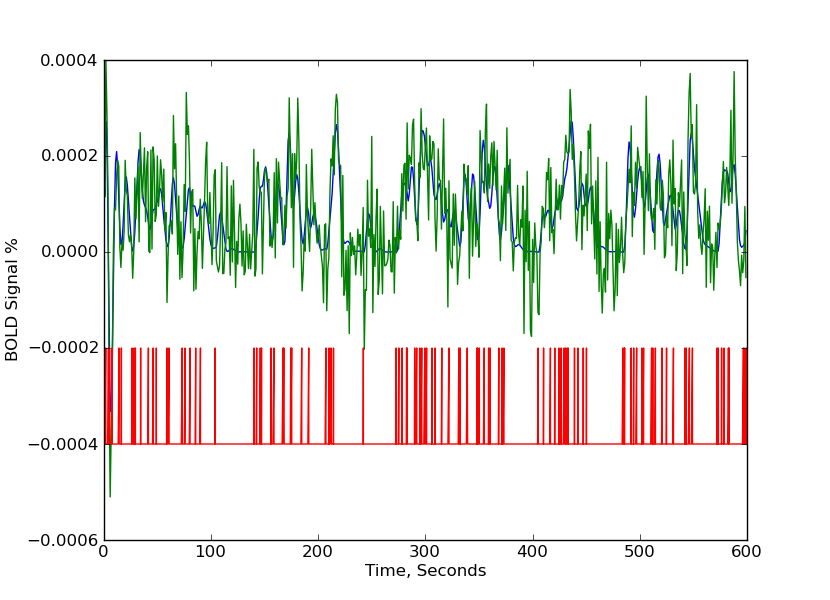
\includegraphics[width=8in,height=4in]{noise.png}
\caption{Simulated time-series for a single region. The red line
shows the input stimulus, the blue line shows the base BOLD 
response, and the green line is the BOLD response with Gaussian
white noise added at SNR of 2}
\label{fig:noise}
\end{figure}

%figure 2
\begin{figure}
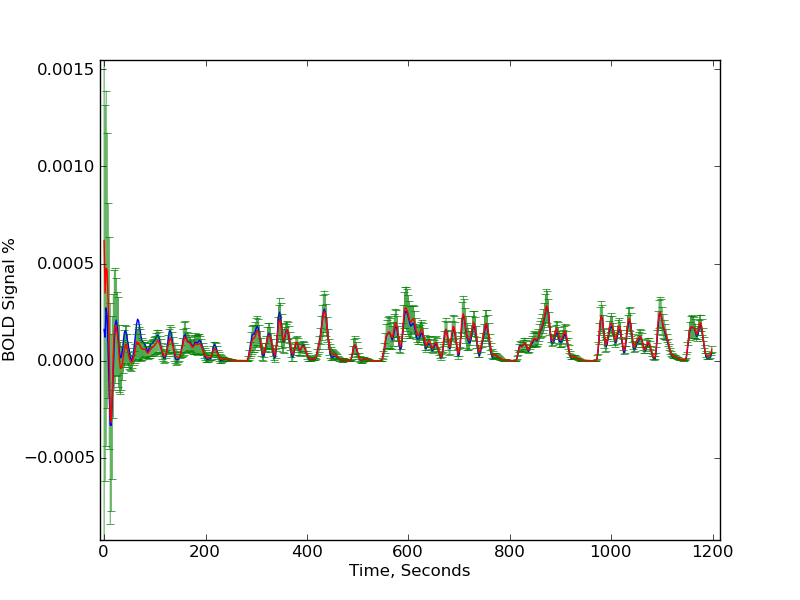
\includegraphics[width=8in,height=4in]{bold.png}
\caption{Particle Filter Results. The blue line is the "true"
(simulated) BOLD response, the red line
is the output of the particle filter with 2 standard deviations
in green. Note that the error bar for time 0 is outside the scope
of the image and is approximately $\pm .003$.}
\label{fig:bold}
\end{figure}

%figure 3
\begin{figure}
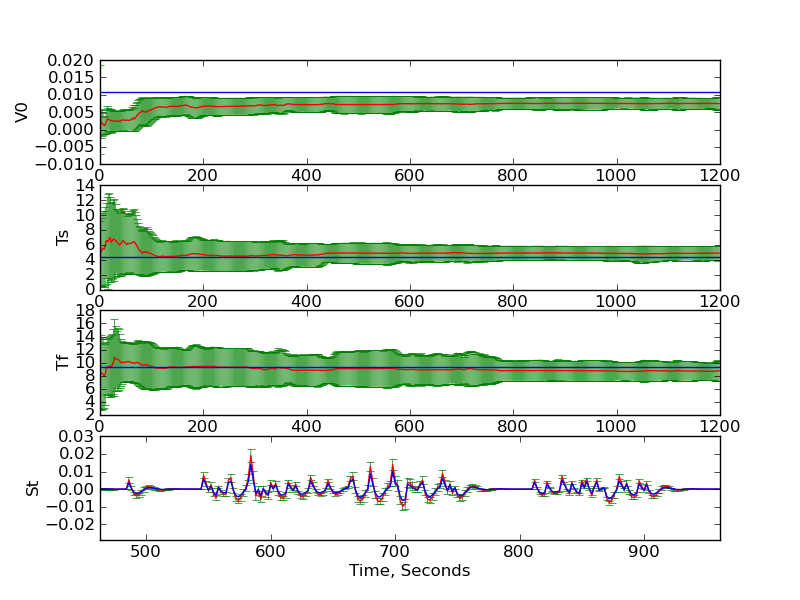
\includegraphics[width=8in,height=4in]{state.png}
\caption{Particle Filter Results. The blue line is the "true"
parameter and the green line is the estimated value for the parameter.
Note that the timescale for $S_t$ is different to highlight an typical
stimulus response. Again 2 standard deviations are shown.}
\label{fig:state}
\end{figure}

Figure 2 shows the estimated BOLD response versus the simulated
data (without noise). It is clear that as the estimated BOLD
response converges to the true BOLD as time progresses. This
is because more and more potential states are eliminated by system's
response to new input sequences. Convergence depends highly on 
the input signal and the weighting function thus choice of both
are extremely important. We have found that an impulse train
(emulated with .1 second width square waves) gives a very good
response. It is also important to choose an input with
some longer hold times, at least as long as than the 
expected time constants, which in this case was around 
8 seconds. The weighting function we have chosen is based
on the exponential distribution, with a variance equal to
the RMS of the signal. While it is important to converge
by the end of the time-series, it is often the case that 
converging too fast will harm the state estimation by over-
emphasizing the measurements of single time points. The rate
of convergence is well within control of the user of the 
particle filter based on the weighting function and the frequency
of re-sampling. Note that resampling can cause quantization
errors due to the nature of estimating a long tailed 
distribution with a finite number of samples. 

Figure 3 shows the estimated versus simulated values for
several key parameters. Notice how the variance drops as
the particle filter continues. The parameters shown are
$V_0$ which is a scaling parameter, $\tau_s$, and $\tau_f$
which are both time constants and $s_t$ which is a hidden
state variable, estimating the flow inducing signal. Note that
even though some of the parameters don't converge to the exact
value, that the estimated $s_t$ still matches the true
$s_t$ relatively well. It is often the cast that although a
few parameters don't converge to their true value, one 
parameter may pick up the slack for another. It is of
note that $\tau_s$ and $\tau_f$ do converge at least close
to their true values, because they cannot be determined
from steady state. 

\bibliographystyle{abbrvnat}
\bibliography{proposal_micah}


\end{document}
